\documentclass{article}
\usepackage{multirow}
\usepackage[table,xcdraw]{xcolor}
\usepackage[utf8]{inputenc}
\usepackage[a4paper, total={6in, 8in}]{geometry}
\usepackage{amsmath}
\usepackage{amssymb}
\usepackage{amsthm}
\usepackage{cancel}
\usepackage{caption}
\usepackage{color,soul}
\usepackage{comment}
\usepackage{graphicx}
\usepackage{hyperref}
\usepackage{listings}
\usepackage{outlines}
\usepackage{subcaption}
\usepackage{tcolorbox}


\newcommand{\lands}{\:\land\:}                          % "logical and with spaces". Pone el "y" dejando espacio(mediano) a los costados
\newcommand{\comma}{,\,}                                % Pone la coma seguida de un espacio(chiquito)
\newcommand{\tq}{/\,}                                   % "tal que". Pone la barrita del "tal que" seguida de un espacio
\newcommand{\vees}{\:\vee\:}                            % "vee with spaces". Pone el "ó" con espacio a los costados
\newcommand{\eq}{\:=\:}                                 % Pone el igual con espacios(medianos) a los costados
\newcommand{\neqs}{\:\neq\:}                            % Pone el desigual con espacios(medianos) a los costados
\newcommand{\relates}{\mathcal{R}}                      % Pone la R para denotar cuando un elemento se realciona con otro
\newcommand{\enteros}{\mathbb{Z}}                       % Pone la Z de los números enteros
\newcommand{\naturales}{\mathbb{N}}                     % Pone la N de los números naturales
\newcommand{\racionales}{\mathbb{Q}}                    % Pone la Q de los números racionales
\newcommand{\complejos}{\mathbb{C}}                     % Pone la C de los números complejos
\newcommand{\cuerpo}{\mathbb{K}}                        % Pone la K para denotar un cuerpo (los cuerpos son R,Q o C)
\newcommand{\reales}{\mathbb{R}}                        % Pone la R de los números reales
\newcommand{\partes}{\mathcal{P}}
\newcommand{\vabs}[1]{\left\lvert #1 \right\rvert }     % Pone el módulo y recibe como argumento el número
\newcommand{\Rightarrows}{\: \Rightarrow \:}            % Pone la flecha del "entonces" con espacios(medianos) a los costados
\newcommand{\Leftrightarrows}{\: \Leftrightarrow \:}    % Pone la flecha del "si y solo si" con espacios(medianos)
\newcommand{\existsuniq}{\exists !\,}                   % Pone el "existe un único" dejando un espacio(chiquito) para que no quede tan amontonado
\newcommand{\bld}[1]{\textbf{#1}}
\newcommand{\sumatoria}[2]{\sum_{#1} ^{#2}}
\newcommand{\comb}[2]{{{#1}\choose{#2}}}

\title{Resumen - Probabilidad y Estadística}
\author{Nicolás Margenat}
\date{1Q 2022}

\begin{document}
\maketitle
\tableofcontents

\newpage
\section{Concepto de Probabilidad}
\subsection{Definiciones}
\subsubsection*{Definición 1. Espacio Muestral}
Conjunto de todos los resultados posibles de un determinado experimento.

\subsubsection*{Definición 2. Suceso/Evento}
Conjunto de resultados posibles de un experimento.


\subsection{Álgebra de Sucesos}
\begin{align*}
    E:& \text{ Experimento aleatorio - Resultados inciertos} \\
    S:& \text{ Espacio muestral} \\
    A:& \text{ Suceso o Evento}
\end{align*}
Cabe mencionar que:
\begin{equation*}
    A \subset S
\end{equation*}

\leavevmode\\ Dos sucesos son \textbf{mutuamente excluyentes} sii
\begin{equation*}
    A \cap B = \varnothing
\end{equation*}
es decir, es $imposible$ que sucedan juntos.


\subsection{Frecuencia Relativa de un suceso}
Si un determinado experimento se repite $n$ veces y se cuenta el numero de veces que ocurre $n_A$, entonces
la $frecuencia$ $relativa$ de $A$ viene dada por:
\begin{equation*}
    f(A) = \frac{n_A}{n} \; \in [0;1]
\end{equation*}

\subsubsection{Propiedades}
\begin{enumerate}
    \item $f(A) \in [0;1]$
    \item $f(S) = 1$
    \item Si $A \cap B = \varnothing$, entonces:
    \begin{equation*}
        f(A \cup B) = f(A) + f(B) - f(A \cap B)
    \end{equation*}
\end{enumerate}

\subsection{Probabilidad de un suceso}
\subsubsection{Axiomática de Kolmogorov}
\begin{itemize}
    \item $P(A) \geq 0$ (La probabilidad de un suceso es un numero real no negativo)
    \item $P(S) = 1$
    \item Si $A \cap B = \varnothing$, entonces:
    \begin{equation*}
        P(A \cup B) = P(A) + P(B)
    \end{equation*}
\end{itemize}

\subsubsection{Teoremas}
\begin{enumerate}
    \item $P(A) \leq 1$
    \item $P(\bar{A}) = 1 - P(A)$
    \item $P(\varnothing) = 0$
    \item $P(A \cup B) = P(A) + P(B) - P(A \cap B)$
\end{enumerate}
Con estos axiomas podemos derivar que:
\begin{itemize}
    \item $P(A \cup B \cup C) = P(A) + P(B) + P(C) - P(A \cap B) - P(A \cap C) - P(B \cap C) + P(A \cap B \cap C)$
    \item Si $A \cap B = A \Rightarrows P(A) \leq P(B)$
\end{itemize}

\subsubsection{Equivalencia de Expresiones}
\begin{enumerate}
    \item $B = (\bar{A} \cap B) \cup (A \cap B)$
    \item $A \cup B = A \cup (\bar{A} \cap B)$
\end{enumerate}

\subsubsection{Desigualdad de Bonferroni}
\begin{equation*}
    P(\bigcup^n_{j=1} E_j) \leq \sumatoria{j = 1}{n} P(E_j)
\end{equation*}

\subsection{Regla de Laplace}
\begin{equation*}
    P(A) = \frac{\#A}{\#S} = \frac{\text{numero de casos favorables de A}}{\text{numero total de casos posibles}}
\end{equation*}
\textbf{Importante}: Solo sirve en un espacio muestral finito y equiprobable.


\newpage
\section{Estadística Descriptiva}
\section*{Estadística Descriptiva No Agrupada}
\begin{equation*}
    \{x_i\}^n_{i=1}
\end{equation*}
\subsection{Definiciones (ED No Agrupada)}
\subsubsection{Parámetros de Tendencia Central}
\subsubsection*{Definición 1. Media Muestral o Promedio}
Es un \emph{parámetro de tendencia central}.
\\Se calcula:
\begin{equation*}
    \bar{x} = \frac{1}{n} \sumatoria{i=1}{n} x_i
\end{equation*}
\underline{Observación}: El promedio de los desvíos de los datos respecto de la media SIEMPRE es 0,
entonces habrá datos menores que la media y otro mayores que ella.

\subsubsection*{Definición 2. Mediana}
Es un \emph{parámetro de tendencia central} \emph{posición}.
\\En un ordenamiento de menor a mayor, si el numero de datos es \emph{impar} es el termino central.
Si el numero de datos es \emph{par} la mediana se calcula como el promedio de los dos términos centrales.
\\\underline{Notación}: $m$

\subsubsection*{Definición 3. Cuartiles Primero y Tercero}
Es un \emph{parámetro de tendencia central} \emph{posición}.
\\En un ordenamiento de menor a mayor son mediana de la primera mitad y de la segunda mitad de los datos.
\\\underline{Notación}: $q_1$, $q_3$

\subsubsection{Parámetros de Variabilidad}
\subsubsection*{Definición 4. Rango muestral}
La distancia entre el mínimo y el máximo de los datos muestrales.
Es decir, longitud del intervalo al que pertenece el 100% de los datos.
\\\underline{Notación}: $R$

\subsubsection*{Definición 5. Rango Intercuartílico}
Distancia entre $q_1$ y $q_3$. Es decir, longitud del intervalo al que pertenecen el 50\% central de los datos.
\\\underline{Notación}: $iqr$

\subsubsection*{Definición 6. Desvío Estándar Muestral}
Medida típica de variación de cierto conjunto de datos.
\\Se calcula como:
\begin{equation*}
    s = \sqrt{\frac{1}{n-1} \sumatoria{i=1}{n} (x_i - \bar{x})^2}
\end{equation*}

\subsubsection*{Definición 6. Varianza Muestral}
Es el menor de los promedios de cuadrados de desvíos.
\begin{equation*}
    s^2 = \frac{1}{n-1} \sumatoria{i=1}{n} (x_i - \bar{x})^2
\end{equation*}

\subsubsection{Parámetros de Forma}
\subsubsection*{Definición 7. Coeficiente de Simetria}
Medida típica de simetría de los datos respecto de la media, y es nulo si hay simetría.
Si es positivo se dicen que los datos tienen sesgo positivo y negativo en caso contrario
\\Se calcula como:
\begin{equation*}
    \gamma = \frac{1}{ns^3} \sumatoria{i=1}{n} (x_i - \bar{x})^3
\end{equation*}

\subsubsection*{Definición 8. Coeficiente de Kurtosis}
mide la forma de la distribución de datos en torno del promedio.
Es positivo si los datos tienen alta concentración en torno de la media y negativo en caso contrario.
\\Se calcula como:
\begin{equation*}
    \kappa = \frac{1}{ns^4} \sumatoria{i=1}{n} (x_i - \bar{x})^4 - 3
\end{equation*}

\subsection{Boxplot/Diagrama de caja}

\begin{center}
    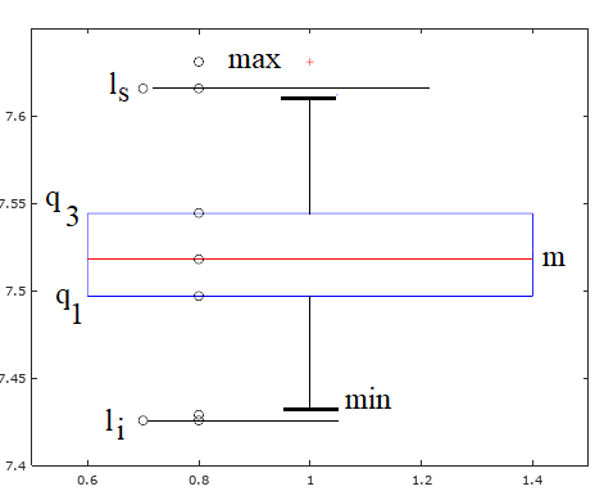
\includegraphics[width=.40\textwidth]{Images/Boxplot.png}
\end{center}

\begin{itemize}
    \item La caja central se determina con $q_1$ y $q_3$
    \item Se representan con dos rayas los datos inmediatos a los limites de Tuckey,
    que se calculan de la siguiente manera:
    \begin{align*}
        l_s =& q_1 + 1,5 * iqr \\
        l_i =& q_1 - 1,5 * iqr
    \end{align*}
    \item Hay \emph{datos outliers} de dos tipos: \textbf{moderados} (tienen un valor menor que $q_1 - 3 * iqr$)
    y \textbf{severos} (tienen valores mayores que $q_3 + 3 * iqr$)
    \begin{center}
        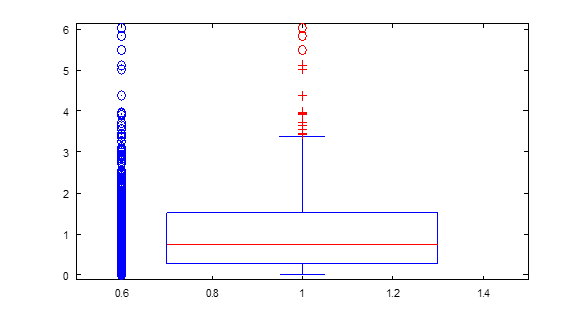
\includegraphics[width=.50\textwidth]{Images/BoxplotModeradosSeveros.png}
        \caption{figure}{+ moderados, O severos}
    \end{center}
    \item Si el máximo o mínimo están antes que el bigote calculado, entonces ahí va el bigote
\end{itemize}

\section*{Estadística Descriptiva Agrupada}
\begin{equation*}
    \{\tilde{x}_r, y_r\}^m_{r=1}
\end{equation*}
\subsection{Definiciones (ED Agrupada)}
\subsubsection*{Defunción 1. Marca de clase}
Es el punto medio del intervalo de clase $r$.
\begin{equation*}
    \tilde{x}_r = \frac{a_r + b_r}{2}
\end{equation*}

\subsubsection*{Definición 2. Frecuencia Absoluta de la clase $r$}
Cantidad de datos del conjunto original que pertenecen al intervalo $r$.

\subsubsection{Parámetros Característicos}
\subsubsection*{Definición 3. Media Muestral o Promedio}
Es un \emph{parámetro de tendencia central}.
\\Se calcula:
\begin{equation*}
    \bar{x} = \frac{1}{n} \sumatoria{r=1}{m} \tilde{x}_r y_r
\end{equation*}

\subsubsection*{Definición 4. Desvío Estándar Muestral}
Medida típica de variación de cierto conjunto de datos.
\\Se calcula como:
\begin{equation*}
    s = \sqrt{\frac{1}{n-1} \sumatoria{r=1}{m} (\tilde{x}_r - \bar{x})^2} y_r
\end{equation*}

\subsubsection*{Definición 5. Coeficiente de Simetria}
Medida típica de simetría de los datos respecto de la media, y es nulo si hay simetría.
Si es positivo se dicen que los datos tienen sesgo positivo y negativo en caso contrario
\\Se calcula como:
\begin{equation*}
    \gamma = \frac{1}{ns^3} \sumatoria{r=1}{m} (\tilde{x}_r - \bar{x})^3 y_r
\end{equation*}

\subsubsection*{Definición 8. Coeficiente de Kurtosis}
mide la forma de la distribución de datos en torno del promedio.
Es positivo si los datos tienen alta concentración en torno de la media y negativo en caso contrario.
\\Se calcula como:
\begin{equation*}
    \kappa = \frac{1}{ns^4} \sumatoria{r=1}{m} (\tilde{x}_r - \bar{x})^4 y_r - 3
\end{equation*}

\subsection{Histogramas}
    \begin{center}
        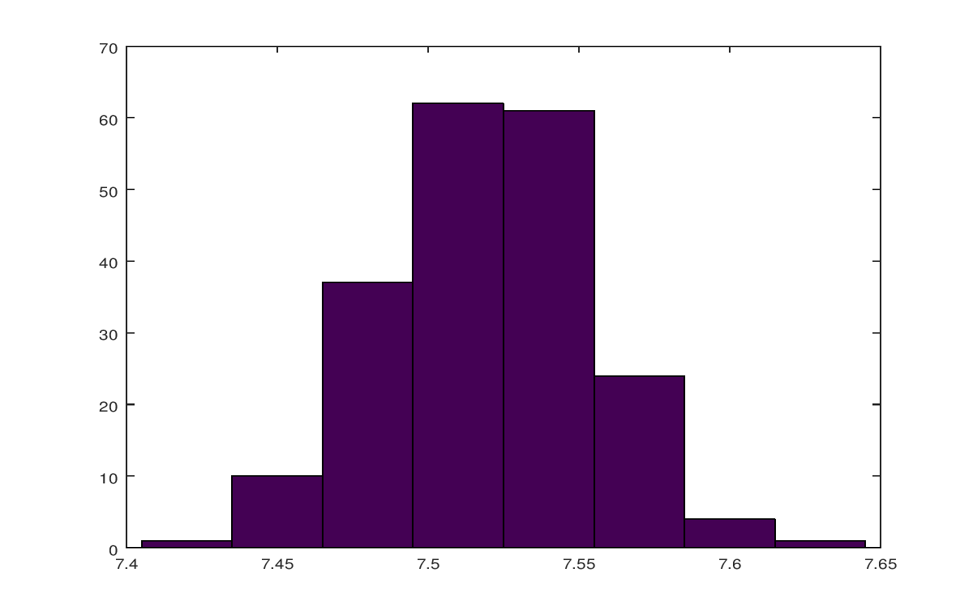
\includegraphics[width=.40\textwidth]{Images/Histogramas.png}
    \end{center}
\begin{itemize}
    \item Cada rectángulo tiene base en un intervalo de clase y la altura mide la frecuencia absoluta del intervalo.
    \item El área del rectángulo es proporcional a $n$ (frecuencia absoluta) y $L$ (longitud de intervalos)
    \item Para elegir el numero de rectángulos, que denominamos $m$, utilizamos la siguiente regla:
    \begin{equation*}
        m = \lceil log_2(n) \rceil
    \end{equation*}
    a partir de este numero podemos sumar o restar un poco para ver si hay un mejor $m$.
    \begin{center}
        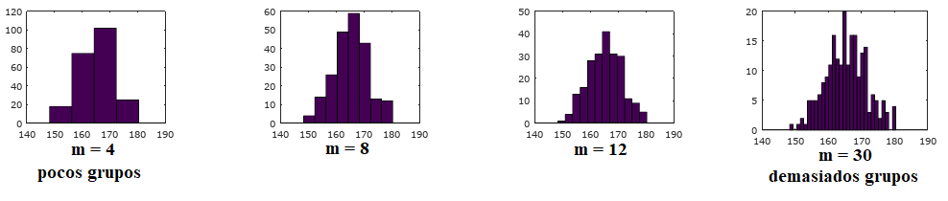
\includegraphics[width=.70\textwidth]{Images/HistogramasM.png}
    \end{center}
\end{itemize}

\subsection{Polígonos}
\subsubsection{Polígono de Frecuencias Absolutas}
    \begin{center}
        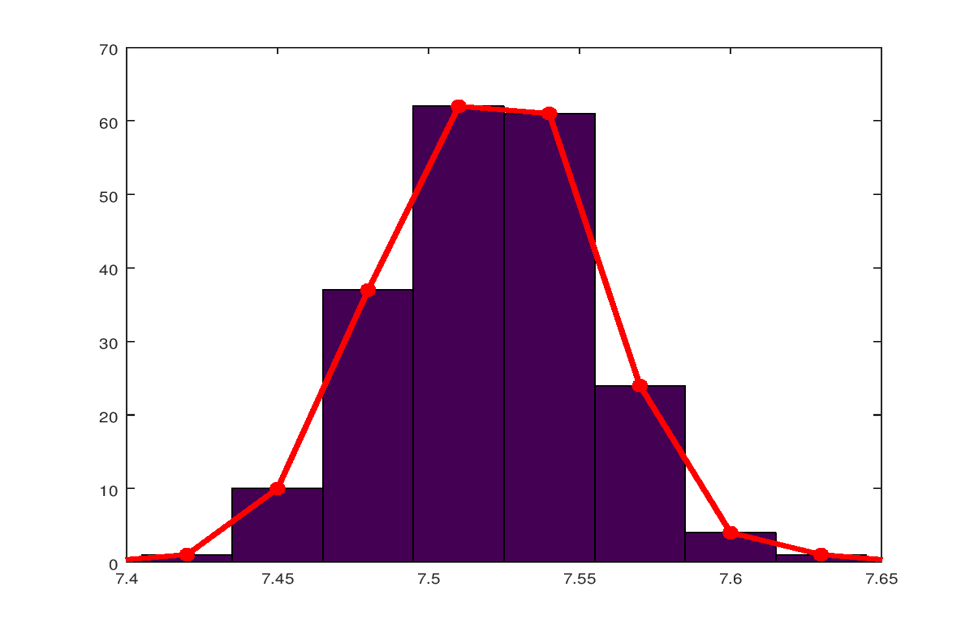
\includegraphics[width=.40\textwidth]{Images/PoligonoFAbs.png}
    \end{center}
    Para construirlo se unen las marcas de clase con lineas rectas, y luego se unen los extremos en donde la ordenada es 0 con las marcas de clase de los extremos.
\subsubsection{Polígono de Frecuencias Relativas}
    \begin{center}
        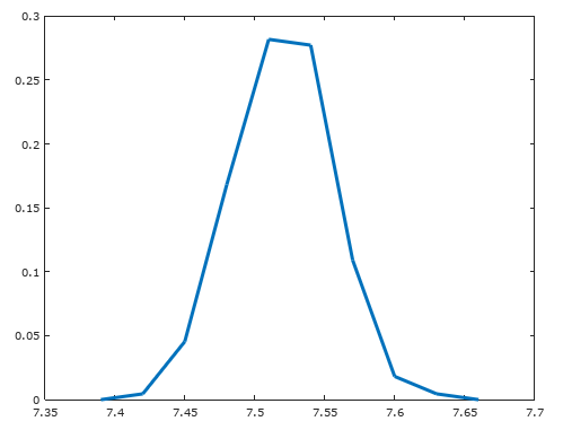
\includegraphics[width=.40\textwidth]{Images/PoligonoFRel.png}
    \end{center}
    Se construye de igual manera que el de frecuencias absolutas, pero usando las frecuencias relativas.
    \\\underline{Observación}: El área bajo este gráfico es $L$, pues la suma de las frecuencias relativas es 1.
\subsubsection{Polígono de Frecuencias Relativas Acumuladas}
    \begin{center}
        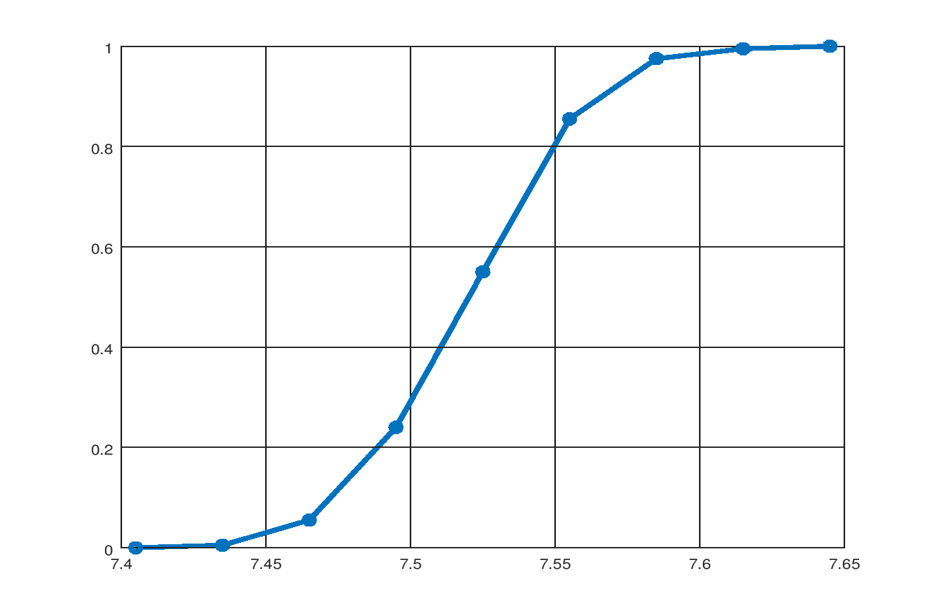
\includegraphics[width=.40\textwidth]{Images/PoligonoFRelAcumuladas.png}
    \end{center}
     Se representa la frecuencia acumulada relativa suponiendo que en cada intervalo la frecuencia aumenta linealmente.
     \\\underline{Observación}: La diferencia de ordenadas en los extremos de un intervalo cualquiera mide la fracción de los datos en ese intervalo.
     
\newpage
\section{Probabilidad Condicional}  
\subsection{Definiciones}
\subsubsection*{Definición 1. $P(A / B)$}
Si $A$ y $B$ son sucesos, y $P(B) > 0$ entonces se introduce la probabilidad condicional de $A$ dado que ocurrió $B$.
\\\underline{Notación}: $P(A / B)$ ("\emph{probabilidad de $A$ dado $B$}")

\subsubsection*{Definición 2. Sucesos independientes}
Dos sucesos son independientes si la probabilidad de que ocurra uno no te influye sobre la probabilidad de otro. Además:
\begin{equation*}
    \text{$A$ y $B$ son independientes} \Leftrightarrows P(A \cap B) = P(A)P(B)
\end{equation*}
Por ejemplo, si tengo un tarro de bolitas con reposición y saco 2 bolitas, después como las bolitas las vuelvo a poner vuelvo a estar en el caso inicial cuando haga la segunda extracción (entonces son sucesos independientes).

\subsection{Propiedades $P(A / B)$}
\begin{enumerate}
    \item $P(A/B) = \frac{P(A \cap B)}{P(B)}$ con $P(B) > 0$
    \item $P(A \cap B) = P(A/B) P(B) = P(B/A) P(A)$ (puedo elegir la que mas me convenga)
    \item Si $A \cap C = \varnothing $
    \begin{equation*}
        \Rightarrows P((A \cup C) / B) = P(A/B) + P(C/B) \text{ con } P(B) > 0
    \end{equation*}
    \item $P(\={A} / B) = 1 - P(A / B)$ pero $P(A / \={B}) \neq 1 - P(A/B)$
    \item $P((A \cup C) / B) = P(A/B) + P(C/B) - P((A \cap C) / B)$
    \item Si $P(A \cap B) = 0 \Rightarrows P(A/B) = 0$
    \item $P(H / E) = \frac{P(H)P(E/H)}{P(E)}$
\end{enumerate}

\subsection{Propiedades Sucesos Independientes}
\begin{enumerate}
    \item Si $A$ y $B$ son independientes, entonces también lo son: $\={A}$ y $B$; $A$ y $\={B}$; y $\={A}$ y $\={B}$
    \item \emph{Condición de independencia para una familia de sucesos}: Sean $\{A_k\}_{k \in K}$ una familia de sucesos independientes, entonces:
    \begin{equation*}
        P(\bigcap_{j \in J} A_j) = \prod_{j \in J} P(A_j) \;\; \forall J \subseteq K
    \end{equation*}
    \subitem Por ejemplo, para el caso de 3 sucesos:
    \begin{center}
        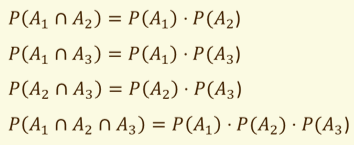
\includegraphics[width=.40\textwidth]{Images/SucIndependientes.png}
    \end{center}    
\end{enumerate}

\subsection{Teoremas}
Sea $S$ un espacio muestral / 
\begin{align*}
    &S = \bigcup_{k=1}^n A_k \\
    &A_k \neq \varnothing \\
    &A_k \cap A_j = \varnothing \text{ si } k \neq j \\
    &B = \bigcup_{k=1}^n ( B \cap A_k ) = \sumatoria{k=1}{n} (B \cap A_k)
\end{align*}
\begin{center}
    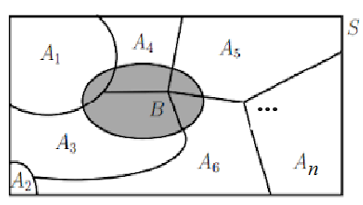
\includegraphics[width=.40\textwidth]{Images/ProbabilidadTotal.png}
\end{center} 
\subsubsection*{Teorema de la Probabilidad Total}
\begin{equation*}
    P(B) = \sumatoria{k=1}{n} P(B / A_k) P(A_k)
\end{equation*}

\subsubsection*{Teorema de Bayes}
\begin{equation*}
    P(A_j/B) = \frac{P(B/A_j)P(A_j)}{\sumatoria{k=1}{n}P(B/A_k)P(A_k)}
\end{equation*}

%-----------------------------------------------------------------------------
\newpage
\section{Variables Aleatorias Discretas}
\subsection{Definiciones}
\subsubsection*{Definición 1. Variable Aleatoria (va)}
Una \emph{variable aleatoria} es la consecuencia numérica de un experimento aleatorio.
\\\underline{Notación}: $X$
\\Ademas, el conjunto de valores posibles de una variable aleatoria es:
\begin{equation*}
    X: S \rightarrow R_X \text{ donde $R_X$ es el recorrido o rango de $X$} 
\end{equation*}
y $S$ es el espacio muestral de un experimento aleatorio.

\subsubsection*{Definición 2. Valor Esperado de una vad}
El \emph{valor esperado de una variable aleatoria} es una medida de centralidad. Nos dice donde se centra la variable considerando las probabilidades.
\\\underline{Notación}: $E(X)$
\begin{equation*}
    E(X) = \sumatoria{x}{} x p_X(x)
\end{equation*}

\subsubsection*{Definición 3. Varianza de una vad}
La varianza de una variable aleatoria una medida de dispersión. Evalúa usando los valores de la probabilidad cuanto se tienden a alejar los valores del recorrido respecto de la media.
\\\underline{Notación}: $V(X)$
\begin{equation*}
    V(X) = \sumatoria{x \in R_X}{} (x - E(X))^2 p_X(x)
\end{equation*}

\subsubsection*{Definición 4. Desvío Estándar de una vad}
El desvío estándar de una variable aleatoria es una medida típica de los desvíos de sus valores respecto del valor esperado.
\\\underline{Notación}: $\sigma(X)$
\begin{equation*}
    \sigma(X) = \sqrt{V(X)}  
\end{equation*}

\subsubsection*{Definición 5. Coeficiente de Simetria de una vad}
\begin{equation*}
    \gamma = \frac{1}{\sigma^3} \sumatoria{x \in R_X}{} (x - E(X))^3 p_X(X)
\end{equation*}

\subsubsection*{Definición 5. Coeficiente de Kurtosis de una vad}
\begin{equation*}
    \gamma = \frac{1}{\sigma^4} \sumatoria{x \in R_X}{} (x - E(X))^4 p_X(X)
\end{equation*}

\subsection{Propiedades}
\subsubsection{Propiedades de $E(X)$}
\begin{enumerate}
    \item $E(a) = a$ si $a$ es una constante
    \item $E(b X) = b E(X)$ si $b$ es una constante
    \item $E(X - E(X)) = 0 \;\; \forall X$
    \item $E(X + Y) = E(X) + E(Y)$
    \item $E(G(X)) = \sumatoria{x \in R_X}{} G(X) p_X (x)$
\end{enumerate}

\subsubsection{Propiedades de $V(X)$}
\begin{enumerate}
    \item $V(X) \geq 0$
    \item $V(a) = 0$ si $a$ es una constante
    \item $V(b X) = b^2V(X)$ si $b$ es una constante
    \item $V(X) = E(X^2) - (E(X))^2$ donde $E(X^2) = \sumatoria{x \in R_X}{} x^2 p_X(x)$
\end{enumerate}

\subsection{VADs Notables}
\subsubsection{VAD Bernoulli}
Caracteriza la ocurrencia o no de un suceso al realizar un experimento aleatorio.
\\\underline{Características}:
\begin{enumerate}
    \item $X \sim Bernoulli(p)$
        \subitem $R_X = \{ 0, 1 \}$ donde $0$ es fracaso y $1$ es éxito
    \item $P(X=1) = p$, $P(X=0) = 1 - p = q$
    \item $E(X) = p$
    \item $V(X) = pq$
\end{enumerate}

\subsubsection{VAD Binomial}
(\textbf{con reposición}) Cuenta el número de ocurrencias de un evento de interés en $n$ de repeticiones \emph{independientes} de un experimento aleatorio con igual probabilidad $p$ de éxito. 
\\\underline{Características}:
\begin{enumerate}
    \item $X \sim Binomial(n,p)$
        \subitem $R_X = \{0,1,...,n\}$
    \item $P(X = k) = {{n}\choose{k}} p^k q^{n-k} \;\; \forall k \in R_X$
    donde  
        \subitem ${{n}\choose{k}}$: formas de elegir las posiciones de los éxitos
        \subitem $p^k$:  probabilidad de $k$ éxitos 
        \subitem $q^{n-k}$: probabilidad de $n-k$ fracasos
    \item $E(X) = np$
    \item $V(X) = np(1-p)$
\end{enumerate}
donde $X =$ número de éxitos en los $n$ experimentos.

\subsubsection{VAD Hipergeométrica}
(\textbf{sin reposición}) Cuenta el número de elementos de cierta clase en una muestra aleatoria extraída sin reposición de una población que contiene elementos de esa clase. 
\\\underline{Ejemplo}: Población de $N$ individuos divididos en 2 clases $A$ y $B$. La $A$ tiene $M$ individuos y la $B$ tiene $N-M$. Se toma una muestra de $n$ individuos sin reposición.
\\\underline{Características}:
\begin{enumerate}
    \item $X \sim Hipergeométrica(N,M,n)$
        \subitem $R_X = max(0, n - (N - M)) \leq k \leq min(M,n)$
    \begin{center}
        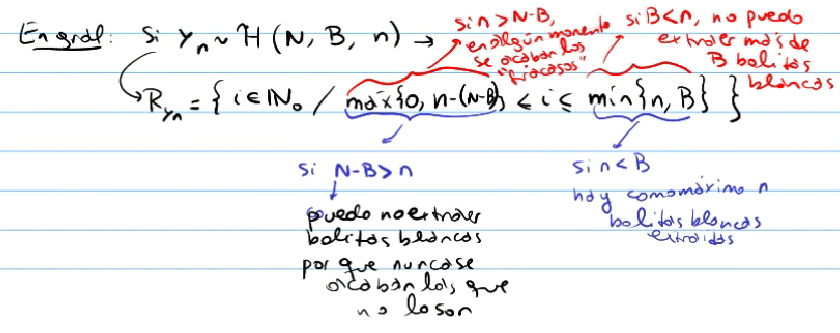
\includegraphics[width=.60\textwidth]{Images/VADHipRx.png}
    \end{center} 
    \item $P(X=k) = \frac{\comb{M}{k} \comb{N-M}{n-k}}{\comb{N}{n}}$ donde $max(0, n - (N - M)) \leq k \leq min(M,n)$
    \item $E(X) = n \frac{M}{N}$
    \item $V(X) = n \frac{M}{N} \frac{N-M}{N} \frac{N-n}{N-1}$
\end{enumerate}
\underline{Observación}: Si hay mas de 2 clases estas reglas ya no se cumplen.
\\\textbf{Relación con la binomial}: 
\begin{equation*}
    X \sim Hipergeométrica(N, M, n), \; Y \sim Binomial(n ,\frac{M}{N}) \Rightarrows P(X \leq k) \approx P(Y \leq k)
\end{equation*}

\subsubsection{VAD Geométrica}
(\textbf{con reposición}) Cuenta el número de repeticiones \emph{independientes} de un experimento aleatorio hasta la primera ocurrencia de un evento de interés. 

\begin{enumerate}
    \item $X \sim Geom(p)$
        \subitem $R_X = \{ 1, 2, ... \} = \naturales$

    \item $P(X = k) = (1 - p)^{k-1} p \;\; \forall k \in R_X$
    \item $E(X) = \frac{1}{p}$
    \item $V(X) = \frac{1-p}{p^2}$
\end{enumerate}
donde $X =$ numero de intentos hasta el primer éxito (\textbf{incluido}).
\subsubsection*{Propiedades}
\begin{itemize}
    \item $P(X > M) = 1 - P(X \leq M) = (1 - p)^m$
    \item $P(X > M + N | X > M) = P(X > N)$ ("\emph{falta de memoria}")
\end{itemize}



\subsubsection{VAD Poisson}
Asociada a un especial proceso denominado de Poisson.  Acá la vamos a usar como aproximación a la distribución binomial.
\\Se cuenta la cantidad de veces que ocurre algo, pero a diferencia de la binomial, estos eventos no tienen cantidad máxima. La ventaja de Poisson es que tiene un parámetro, mientras que la binomial tiene 2. Entonces nos puede servir cuando no se sabe $n$, ni $p$, pero se sabe el valor esperado $\lambda$ (y $n$ es grande y $p$ es pequeño).
\underline{Características}:
\begin{enumerate}
    \item $X \sim Poisson(\lambda)$ con $\lambda > 0$
        \subitem $R_X = \{ 0,1,...\} = \naturales_0$
    \item $P(X=k) = \frac{\lambda^k}{k!}e^{-\lambda}$ $\forall k \in R_X$
    \item $E(X) = \lambda$
    \item $V(X) = \lambda$
\end{enumerate}
\underline{Observación}: Si $\lambda \in \naturales$ entonces tiene 2 valores máximos ($\lambda$ y $\lambda - 1$). En cambio, si $\lambda \in \reales - \naturales$ entonces tiene 1 valor máximo ($\lfloor \lambda \rfloor$).

\subsection{Función Distribución de una vad $X$}
Llamamos Función Distribución a $F: \reales \rightarrow [0,1] \tq$
\begin{equation*}
    F_X(x) = P(X \leq x) = \sumatoria{t \leq x0}{} p_X(t)
\end{equation*}
\subsubsection*{Propiedades}
\begin{enumerate}
    \item $\lim_{x \rightarrow \infty} F(x) = 1$
    \item $\lim_{x \rightarrow -\infty} F(x) = 0$
    \item $x_1 < x_2 \Rightarrows F(x_1) < F(x_2)$ (creciente)
    \item $P(a < X \leq b) = F_X(b) - F_X(a)$
\end{enumerate}

\newpage
\section{Variables Aleatorias Continuas}
Son variables aleatorias cuyo rango es un intervalo de números reales o una unión de intervalos reales.
\begin{equation*}
    X: S \rightarrow R_X \subseteq \reales
\end{equation*}
Aquí, $P(X = a) = 0$.
\subsection{Definiciones}
\subsubsection*{Definición 1. Valor Esperado de una vac}
Se define como: 
\begin{equation*}
    E(X) = \int_{-\infty}^{+\infty} xf_X(x) dx
\end{equation*}

\subsubsection*{Definición 2. Varianza de una vac}
Se define como:
\begin{equation*}
    V(X) = E(X^2) - (E(X))^2
\end{equation*}
donde $E(X^2) = \int^{\infty}_{-\infty} x^2 f(x) dx$

\subsubsection*{Definición 3. Desvío estándar de una vac}
Se define como:
\begin{equation*}
    \sigma(X) = \sqrt{V(X)}
\end{equation*}
\underline{Observación}: Si el valor esperado y el desvío de X son finitos con ambos se puede construir un intervalo  en el que la probabilidad de que X tome valores en él es significativamente grande.

\subsubsection*{Definición 4. Momentos de una va}
Se definen dos momentos:
\begin{enumerate}
    \item \textbf{Momento Absoluto de orden $n$}: $M_n = E(X^n)$
    \item \textbf{Momento Centrado de orden $n$}: $\mu_n = E((X - E(X))^n$
\end{enumerate}
con $n \in \naturales_0$

\subsubsection*{Definición 5. Coeficiente de Simetría de una vac}
Se define como:
\begin{equation*}
    \gamma = \frac{\mu_3}{\sigma(X)^3}
\end{equation*}
    \begin{center}
        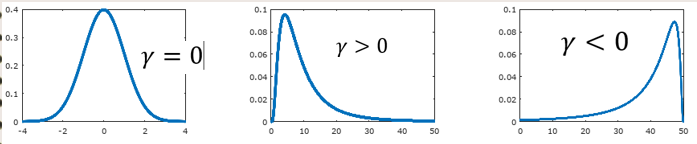
\includegraphics[width=.60\textwidth]{Images/CoefSimetriaVAC.png}
    \end{center} 

\subsubsection*{Definición 6. Coeficiente de Kurtosis de una vac}
Se define como:
\begin{equation*}
    \gamma = \frac{\mu_4}{\sigma(X)^4}
\end{equation*}
\begin{center}
        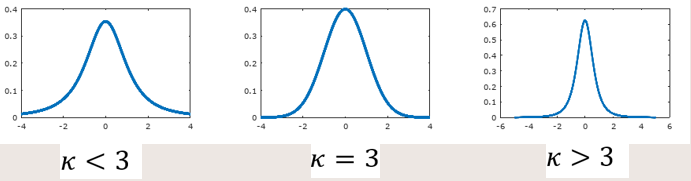
\includegraphics[width=.60\textwidth]{Images/CoefKurtosisVAC.png}
    \end{center} 

\subsection{Función de Densidad de Probabilidad de $X$}
Se define como:
\begin{equation*}
    F_X(x) = P(a < X < b) = \int_a^b f_X(x)
\end{equation*}

\subsubsection*{Propiedades}
\begin{enumerate}
    \item $\int^\infty_{-\infty} f_X(x) dx = 1$
    \item $\lim_{x \rightarrow +\infty} F(X) = 1$
    \item $\lim_{x \rightarrow -\infty} F(X) = 0$
\end{enumerate}

\subsection{Función Distribución de una vac $X$}
Llamamos Función Distribución a $F: \reales \rightarrow [0,1] \tq$
\begin{equation*}
    F_X(x) = P(X \leq x) = \int_{-\infty}^x f_X(t) dt
\end{equation*}
\subsubsection*{Propiedades}
\begin{enumerate}
    \item $\lim_{x \rightarrow \infty} F(x) = 1$
    \item $\lim_{x \rightarrow -\infty} F(x) = 0$
    \item $x_1 < x_2 \Rightarrows F(x_1) < F(x_2)$ (creciente)
    \item $P(a < X < b) = F_X(b) - F_X(a)$
    \item $F'_X(x) = f_X(x)$ (continua)
\end{enumerate}



\subsection{VACs Notables}
\subsubsection{VAC con Distribución Uniforme}
\begin{equation*}
    X \sim U(a,b)
\end{equation*}
Una vac tiene \emph{distribución uniforme} en el intervalo $(a,b)$ si:
\begin{equation*}
    f_X(x) =\left\{ \begin{array}{lcc}
             \frac{1}{b-a}&  \text{si } x \in (a,b) \\
             \\ 0 & \text{si } x \notin (a,b)
             \end{array}
   \right.
\end{equation*}
\begin{center}
        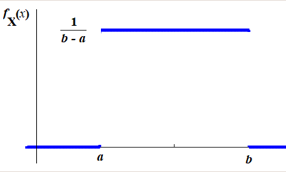
\includegraphics[width=.30\textwidth]{Images/VACUnif.png}
    \end{center} 
Luego, si una vac tiene \emph{distribución uniforme}, entonces:
\begin{equation*}
    F_X(x) =\left\{ \begin{array}{lcc}
             0&  \text{si } x \leq a \\
             \\ \frac{x-a}{b-a}& \text{si } x \in (a,b) \\
             \\ 1& \text{si } x \geq b
             \end{array}
   \right.
\end{equation*}
\begin{center}
        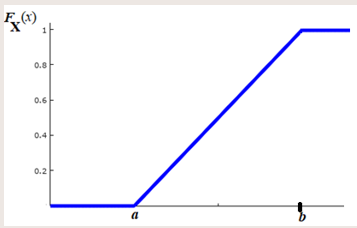
\includegraphics[width=.30\textwidth]{Images/VACUnif2.png}
    \end{center} 
\subsubsection*{Propiedades}
\begin{enumerate}
    \item $E(X) = \frac{a+b}{2}$
    \item $V(X) = \frac{(b-a)^2}{12}$
\end{enumerate}

\subsubsection{VAC con Distribución Exponencial}
\begin{equation*}
    X \sim E(\lambda) \text{ con } \lambda > 0
\end{equation*}
Una vac tiene \emph{distribución exponencial} de parámetro $\lambda > 0$ si:
\begin{equation*}
    f_X(x) =\left\{ \begin{array}{lcc}
             \lambda e^{-\lambda x}&  \text{si } x > 0 \\
             \\ 0 & \text{si } x \leq 0
             \end{array}
   \right.
\end{equation*}
\begin{center}
        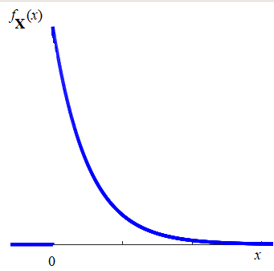
\includegraphics[width=.25\textwidth]{Images/VACExp.png}
    \end{center} 
Luego, si una vac tiene \emph{distribución exponencial}, entonces:
\begin{equation*}
    F_X(x) = P(X \leq x) =\left\{ \begin{array}{lcc}
             0&  \text{si } x \leq 0 \\
             \\ 1 - e^{-\lambda x}& \text{si } x > 0
             \end{array}
   \right.
\end{equation*}
\begin{center}
        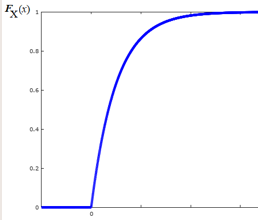
\includegraphics[width=.25\textwidth]{Images/VACExp2.png}
    \end{center} 
de donde podemos obtener que:
\begin{equation*}
    f_X(x) = P(X \geq x) = 1 - F_X(x) = \left\{ \begin{array}{lcc}
             1&  \text{si } x \leq 0 \\
             \\ e^{-\lambda x}& \text{si } x > 0
             \end{array}
   \right.
\end{equation*}


\subsubsection*{Propiedades}
\begin{enumerate}
    \item $E(X) = \frac{1}{\lambda}$
    \item $E(X^n) = \frac{n!}{\lambda^n}$ con $n \in \naturales$
    \item $V(X) =  \frac{1}{\lambda^2}$
    \item $\sigma(X) = E(X) = \frac{1}{\lambda}$
    \item $P(X > a + d | X > a) = P(X > d)$ ("\emph{falta de memoria}"), es decir tiene que ver con la longitud del intervalo
\end{enumerate}

\subsubsection{VAC con Distribución Normal}
\begin{equation*}
    X \sim N(\mu, \sigma)
\end{equation*}
Una vac tiene \emph{distribución normal} si:
\begin{equation*}
    f_X(x) = \frac{1}{\sqrt{2 \pi} \sigma} e^{-\frac{1}{2}(\frac{x - \mu}{\sigma})^2}
\end{equation*}
donde $\mu$ es \emph{media, mediana y modo} y $\sigma$ es el \emph{desvío estándar}.
\begin{center}
        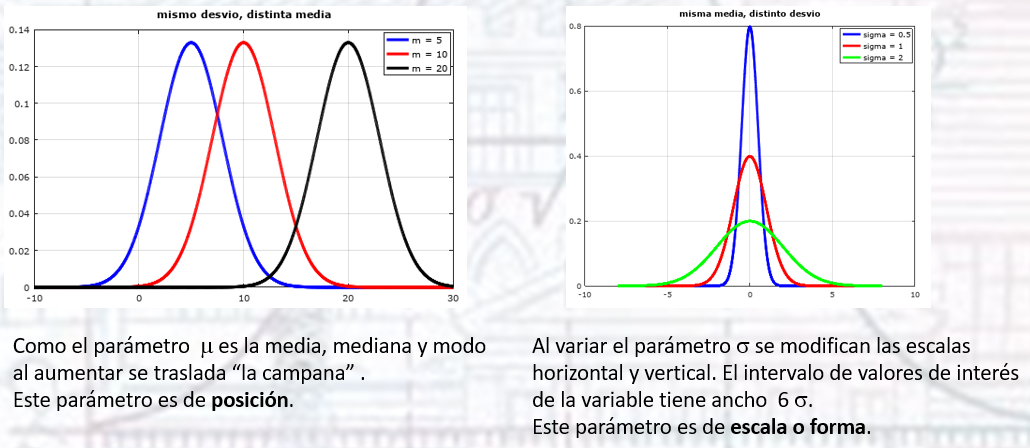
\includegraphics[width=.70\textwidth]{Images/DistribucionNormalVAC.png}
\end{center} 

\subsubsection*{Propiedades A}
\begin{enumerate}
    \item $E(X) = \mu$
    \item $\gamma(X) = 0$
    \item $V(X) = \sigma^2$
    \item $\sigma(X) = \sigma$
    \item $\kappa(X) = 3$ (esto es sin restarle 3)
\end{enumerate}

\subsubsection*{Propiedades B}
\begin{enumerate}
    \item $f(x) > 0 \;\; \forall x \in \reales$
    \item $\lim_{|x| \rightarrow \infty} f_X(x) = 1$
    \item $\int^\infty_{-\infty} f_X(x) = 1$
    \item $f_X(\mu + d) = f_X(\mu - d) \;\; \forall d$
    \item $\int^\mu_{-\infty} f_X(x) = \int^\infty_{\mu} f_X(x) = 0,5$
    \item $f_X'(x) = f_X''(x) = 0$
    \item $P(a < X < b) = \int_a^b f_X(x) dx = F_X(b) - F_X(a)$
\end{enumerate}

\subsubsection*{Cálculo de probabilidad en un intervalo}
\begin{enumerate}
    \item Estandarizamos la variable $X$, para ello tomamos $Z = \frac{X - \mu}{\sigma}$:
    \begin{equation*}
        F_X(x) = \frac{1}{\sqrt{2 \pi} \sigma} \int^x_{-\infty} e^{-\frac{1}{2}(\frac{x - \mu}{\sigma})^2} dx \Rightarrows F_X(x) = \frac{1}{\sqrt{2 \pi}} \int^{\frac{x- \mu}{\sigma}}_{-\infty} e^{-\frac{z^2}{2}} dz = \Phi\left(\frac{x - \mu}{\sigma}\right)
    \end{equation*}
    \item $P(a < X < b) = P(\frac{a - \mu}{\sigma} < Z < \frac{b - \mu}{\sigma}) = \Phi(\frac{b - \mu}{\sigma}) - \Phi(\frac{a - \mu}{\sigma})$ y usando la tabla o una calculadora calculamos.
\end{enumerate}

\subsubsection*{Propiedades C}
\begin{enumerate}
    \item $P(Z < -z) = P(Z > z) = 1 - P(Z < z)$
    \item $\Phi(-z) = 1 - \Phi(z)$
    \item $P(-a < Z < a) = \Phi(a) - \Phi(-a) = 2\Phi(a) - 1$
\end{enumerate}
\textbf{No resumí fractiles porque no entendí nada.}

\subsection{Intervalo de Interés}
Tomamos el intervalo:
\begin{equation*}
    p = P(E(X) - 3 \sigma(X) < X < E(X) + 3 \sigma(X))
\end{equation*}
\begin{center}
        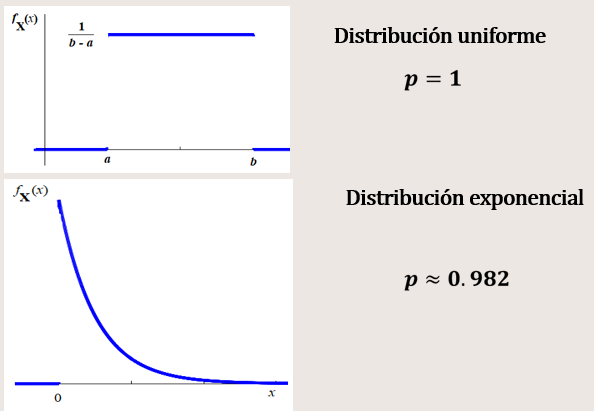
\includegraphics[width=.50\textwidth]{Images/IntervaloInteres.png}
    \end{center} 
Es decir, con este intervalo podemos encapsular prácticamente todo el intervalo de la función probabilidad. De hecho, la probabilidad de que la variable aleatoria tome valores en dicho intervalo es siempre $\geq \frac{8}{9}$.


\newpage
\section{Variables Aleatorias Bidimensionales (VA2D)}
Sean 
\begin{align*}
    &X: S \rightarrow R_X \\
    &Y: S \rightarrow R_Y
\end{align*}
variables aleatorias definidas en el espacio muestral de un experimento aleatorio.
\\Entonces decimos que el par $(X,Y)$ es una VA2D. Además, el \emph{recorrido} de $(X,Y)$ es:
\begin{equation*}
    R_{X,Y} = \{ (x \comma y) \in R_X \times R_Y \tq \exists s \in S: x = X(s) \lands y = Y(s) \} \subseteq R_X \times R_Y
\end{equation*}
\subsubsection*{Propiedades}
\begin{enumerate}
    \item $E(X + Y) = E(X) + E(Y)$
    \item $Cov(X \comma Y) = E((X - E(X))(Y - E(Y)))$
    \item $V(X + Y) = V(X) + V(Y) + 2Cov(X \comma Y)$
\end{enumerate}

\subsubsection*{Propiedades si son INDEPENDIENTES}
\begin{enumerate}
    \item $E(XY) = E(X) E(Y)$
    \item $Cov(X \comma Y) = 0$
    \item $V(X + Y) = V(X) + V(Y)$
\end{enumerate}

\subsubsection{Covarianza}
\begin{enumerate}
    \item $Cov(X \comma Y) = Cov(Y \comma X)$
    \item $Cov(X \comma C) = 0$ si $C$ es constante
    \item $Cov(X \comma X) = V(X)$
    \item $Cov(X \comma Y) = E(XY) - E(X) E(Y)$ ("\emph{fórmula reducida de cálculo de la covarianza}")
    \item $Cov(aX \comma bY) = ab \, E(XY) - E(X) E(Y)$
    \item $Cov(X \comma Y) \neq 0 \Rightarrows X$ e $Y$ son \emph{dependientes}
\end{enumerate}

\subsubsection{Coeficiente de Correlación (lineal) de dos va2d}
Se define como:
\begin{equation*}
     \rho(X \comma Y) = \frac{Cov(X \comma Y)}{\sigma(X) \sigma(Y)}
\end{equation*}
donde $\rho(X \comma Y) \in [-1 \comma 1]$
\subsubsection*{Propiedades}
\begin{enumerate}
    \item $\rho(X \comma Y) = \rho(Y \comma X)$
    \item $\rho(X \comma X) = 1$
    \item $\rho(X \comma C) = 0$ si $C$ es constante
    \item $ab > 0 \Rightarrows \rho(aX \comma bY) = \rho(X \comma Y)$
    \item Si existen constantes $a \neq 0 \comma b$ y $Y = aX + b \Leftrightarrows \rho(X \comma Y) = sign(a) = \left\{ \begin{array}{lcc}
         1& \text{si } a > 0 \\
         -1& \text{si } a < 0
    \end{array}
    \right.$ 
\end{enumerate}
\subsection{VA2D Discretas}
Cuando los recorridos de ambas variables es \emph{discreto} entonces el recorrido de la va2d es discreto.

\subsubsection{Función de Probabilidad Conjunta}
Se define como:
\begin{equation*}
    p_{XY}: R_{XY} \rightarrow [0 \comma 1 ] \tq p_{XY}(x \comma y) = P(X = x \comma Y = y) = \left\{ \begin{array}{lcc}
         0& \text{ si } (x \comma y) \notin R_{XY}  \\
         p_{XY}(x \comma y) > 0&  \text{ si } (x \comma y) \in R_{XY}
    \end{array} 
    \right.
\end{equation*}

\subsubsection{Cálculo de Probabilidades de Sucesos}
\begin{equation*}
    P(A) = P((X\comma Y) \in A) = \sumatoria{(x,y) \in A}{} \sumatoria{}{} p_{XY}(x \comma y)
\end{equation*}

\subsubsection{Valores Esperados de Funciones de X e Y}
\begin{equation*}
    E(G(X \comma Y)) = \sumatoria{(x \comma y) \in R_{XY}}{} \sumatoria{}{} G(x \comma y) p_{XY}(x \comma y)
\end{equation*}

\subsubsection{Distribuciones de Probabilidad de Funciones de X e Y}
Tomo $Z = G(x \comma y)$. Entonces:
\begin{equation*}
    F_Z(z) = P(Z \leq z) = \sumatoria{G(x,y) \leq z}{} \sumatoria{}{} p_{XY}(x \comma y)
\end{equation*}

\subsubsection{Funciones de Probabilidad Marginales}
\begin{equation*}
    \begin{array}{lcc}
     & p_X(x) = \sumatoria{y \in R_Y}{} p_{XY}(x \comma y)  &(1)\\
     \\
     & p_Y(y) = \sumatoria{x \in R_X}{} p_{XY}(x \comma y)  &(2)
\end{array}
\end{equation*}
En (1) la variable $x$ está fija, y solo varía la $y$. En (2) la variable $y$ está fija, y solo varía la $x$.

\subsubsection{Función de Probabilidad Condicional}
\begin{equation*}
    \begin{array}{lcc}
     & p_{X|Y=y}(x,y) = \frac{p_{XY}(x,y)}{p_Y(y)}  &\text{con } p_Y(y) \neq 0\\
     \\
     & p_{Y|X=x}(x,y) = \frac{p_{XY}(x,y)}{p_X(x)} &\text{con } p_X(x) \neq 0
\end{array}
\end{equation*}

\subsubsection{Generalización de Probabilidad de Intersección}
\begin{equation*}
    p_{XY}(x \comma y) = p_{X|Y=y}(x,y)p_Y(y) = p_{Y|X=x}(x,y)p_X(x)
\end{equation*}

\subsubsection{Independencia de VA2D Discretas}
Dos va2d discretas son independientes sii:
\begin{equation*}
    p_{XY}(x \comma y) = p_X(x) p_Y(y) \;\; \forall x \comma y
\end{equation*}

\subsection{VA2D Continuas}
Cuando el recorrido de ambas variables son intervalos reales, o unión de ellos, entonces la va es \emph{continua}.

\subsubsection{Función de Densidad de Probabilidad Conjunta}
\begin{equation*}
    P(A) = \int \int_A f_{X , Y} (x \comma y) dx dy
\end{equation*}
\subsubsection*{Propiedades}
\begin{enumerate}
    \item $f_{X , Y} (x \comma y) \geq 0 \;\; \forall (x \comma y) \in \reales^2$
    \item $\int \int_{\reales^2} f_{X , Y} (x \comma y) dx dy = 1$
\end{enumerate}

\subsubsection{Cálculo de Probabilidades de Sucesos}
\begin{equation*}
    P(A) = P((X\comma Y) \in A) = \int \int_{(x,y) \in A}f_{X,Y}(x \comma y) dxdy
\end{equation*}

\subsubsection{Valores Esperados de Funciones de X e Y}
\begin{equation*}
    E(G(X \comma Y)) = \int \int_{\reales^2} G(x,y) f_{X,Y}(x \comma y) dxdy
\end{equation*}

\subsubsection{Distribuciones de Probabilidad de Funciones de X e Y}
Tomo $Z = G(x \comma y)$. Entonces:
\begin{equation*}
    F_Z(z) = P(Z \leq z) = \int \int_{A_Z}f_{X,Y}(x \comma y) dxdy
\end{equation*}
donde $A_Z = \{(x \comma y) \tq G(x \comma y) \leq z\}$

\subsubsection{Funciones de Densidad de Probabilidad Marginales}
\begin{equation*}
    \begin{array}{lcc}
     & f_X(x) = \int_{- \infty}^\infty f_{X , Y} (x \comma y) \, dy  &(1)\\
     \\
     &  f_Y(y) =\int_{- \infty}^\infty f_{X , Y} (x \comma y) \, dx  &(2)
\end{array}
\end{equation*}
En (1) la variable $x$ está fija, y solo varía la $y$. En (2) la variable $y$ está fija, y solo varía la $x$.

\subsubsection{Función de Densidad de Probabilidad Condicional}
\begin{equation*}
    \begin{array}{lcc}
     & f_{X|Y=y}(x,y) = \frac{f_{XY}(x,y)}{f_Y(y)}  &\text{con } f_Y(y) > 0\\
     \\
     & f_{Y|X=x}(x,y) = \frac{f_{XY}(x,y)}{f_X(x)} &\text{con } f_X(x) > 0
\end{array}
\end{equation*}

\subsubsection{Generalización de Probabilidad de Intersección}
\begin{equation*}
    f_{XY}(x \comma y) = f_{X|Y=y}(x,y)f_Y(y) = f_{Y|X=x}(x,y)f_X(x)
\end{equation*}

\subsubsection{Independencia de VA2D Continuas}
Dos va2d continuas son independientes sii:
\begin{equation*}
    f_{XY}(x \comma y) = f_X(x) f_Y(y) \;\; \forall (x \comma y) \in \reales^2
\end{equation*}

%----------------------------------------------------
\newpage
\section{Suma de Variables Independientes Idénticamente Distribuidas}
Sean $X \comma Y$ va iid con $E(X) = \mu$ y $V(X) = \sigma^2$. Entonces:
\begin{enumerate}
    \item $E(X + Y) = 2\mu$
    \item $V(X + Y) = 2\sigma^2$
    \item $E(\sumatoria{i=1}{n} X_i) = n \mu$
    \item $V(\sumatoria{i=1}{n} X_i) = n \sigma^2$
    \item $E(\={X}_n) = \mu$ donde $\={X}_n = \frac{1}{n}\sumatoria{n}{i=1} X_i$ (promedio)
    \item $E(\={X}_n) = \frac{\sigma^2}{n}$ donde $\={X}_n$ es el promedio
\end{enumerate}

\subsubsection*{Casos Especiales}
\begin{enumerate}
    \item $X_1 \sim Bin(n_1 \comma p) \comma X_2 \sim Bin(n_1 \comma p)$
    \begin{equation*}
    \Rightarrows X_1 + X_2 \sim Bin(n_1 + n_2 \comma p)
    \end{equation*}
    
    \item $X_1 \sim Poiss(\lambda_1) \comma X_2 \sim Poiss(\lambda_2)$
    \begin{equation*}
        \Rightarrows X_1 + X_2 \sim Poiss(\lambda_1 + \lambda_2)
    \end{equation*}
    
    \item $X_1 \sim N(\mu_1 \comma \sigma_1) \comma X_2 \sim N(\mu_2 \comma \sigma_2)$
    \begin{equation*}
        \Rightarrows X_1 + X_2 \sim N\left(\mu_1 + \mu_2 \comma \sqrt{\sigma_1^2 + \sigma_2^2}\right)
    \end{equation*}
    
    \item $X_1 \comma X_2 \comma ... \comma X_n$ va iid con $X_i \sim Bernoulli(p)$
    \begin{equation*}
        \sumatoria{i=1}{n} X_i \sim Bin(n,p)
    \end{equation*}
    
    \item $X_1 \comma X_2 \comma ... \comma X_n$ va iid con $X_i \sim Exp(\lambda)$
    \begin{equation*}
        S_n = \sumatoria{i=1}{n} X_i \sim Gamma(n \comma \lambda)
    \end{equation*}
    donde $f_{S_n}(t) = \frac{\lambda(\lambda t)^{n-1}e^{-\lambda t}}{(n-1)!}$
\end{enumerate}

\subsection{Teorema Central del Límite}
Sean $X_1 \comma X_2 \comma ... X_n$ va iid con $E(X_1) = \mu$ y $V(X_1) = \sigma^2$. Luego para $n$ grande se tiene que:
\begin{align*}
    \={X}_n &\approx N\left(\mu \comma \frac{\sigma}{\sqrt{n}}\right) \\
    \sumatoria{i=1}{n} X_i &\approx N\left(n \mu \comma \sqrt{n} \sigma\right)
\end{align*}

\subsubsection*{Ejemplos}
\begin{enumerate}
    \item $X_i \sim U(0 \comma 1)$
    \begin{equation*}
        \Rightarrows \={X}_n \approx N\left(0.5 \comma \frac{1}{\sqrt{12n}}\right)
    \end{equation*}
    \item $X_i \sim Bernoulli(p) \comma S_n = \sumatoria{i=1}{n} X_i$
    \begin{equation*}
        \Rightarrows S_n \sim Bin(n \comma p) \approx N(np \comma \sqrt{np(1-p)})
    \end{equation*}
    \item $X_i \sim Exp(\lambda) \comma S_n = \sumatoria{i=1}{n} X_i \sim Gamma(n \comma \lambda)$
    \begin{equation*}
        \Rightarrows S_n \approx N\left(\frac{n}{\lambda} \comma \frac{\sqrt{n}}{\lambda}\right)
    \end{equation*}
\end{enumerate}

\subsection{Ley Débil de los Grandes Números}
Sean $X_1 \comma X_2 \comma ...$ va iid con $E(X_1) = \mu$ y $V(X_1) = \sigma^2$. Entonces:
\begin{equation*}
   lim_{n \rightarrow \infty} P(|\={X}_n - \mu| \geq \epsilon) = 0 \;\; \forall \epsilon
\end{equation*}
\underline{Observación}: Con esta ley, podemos estimar valores medio de va y probabilidades realizando repeticiones independientes de un experimento un gran número de veces.

\subsection{Desigualdad de Markov}
Sea $X$ una va solo \emp{toma valores positivos}. Entonces:
\begin{equation*}
    P(X \geq \alpha) \leq \frac{E(X)}{\alpha}
\end{equation*}

\subsection{Desigualdad de Chebychev}
Sea $X$ una va con $E(X) = \mu$ y $V(X) = \sigma^2$. Entonces:
\begin{equation*}
    P(|X - \mu| \geq \epsilon) \leq \frac{\sigma^2}{\epsilon^2}
\end{equation*}
con $\epsilon > 0$

%-----------------------------------------------------------------
\newpage
\section{Inferencia Estadística}
\subsection{Definiciones}
\subsubsection*{Definición 1. Parámetros poblacionales}
Sea $X$ una variable aleatoria definida en la población. Entonces, los \emph{parámetros de la distribución de probabilidades de $X$} se denominan \emp{parámetros poblacionales}.
\\Toma el valor 1 si sucede $A$, y 0 si no sucede $\Rightarrows P(A) = p$

\subsubsection*{Definición 2. Muestra}
Subconjunto de la población. El muestreo es aleatorio, es decir, todos los miembros de la población tienen la \emph{misma probabilidad} de pertenecer a la muestra.
\\Hay 2 tipos:
\begin{enumerate}
    \item \underline{Muestreo con Reemplazo}: Cada observación se realiza sobre un miembro de la población y se retorna.
    \item \underline{Muestreo sin Reemplazo}: Cada observación se realiza sobre un miembro de la población y no se retorna.
\end{enumerate}

\subsubsection*{Definición 3. Estimador/Estadístico}
Sea $\{ X_1 \comma X_2 \comma ... \comma X_n \}$ una \emph{muestra aleatoria} de tamaño $n$.
\\Toda función real de la muestra aleatoria define una va que se denomina \emp{estimador/estadístico}.
\begin{equation*}
    T = H(X_1 \comma X_2 \comma ... \comma X_n)
\end{equation*}
Los estimadores son \textbf{va, son función de varias va iid}.
\\\underline{Notación}: Decimos que $\hat{\theta}$ es estimador del parámetro poblacional $\theta$.

\subsubsection*{Propiedades deseables}
\begin{enumerate}
    \item \underline{Estimador Insesgado}: $\hat{\theta}$ es un estimador insesgado del parámetro poblacional $\theta$ si
    \begin{equation*}
        E(\hat{\theta}) = \theta
    \end{equation*}
    y quiere decir que las va están centradas en lo que se busca estimar. 
    \\Para ver si un estimador es o no insesgado, es básicamente sacar el valor estimado y ver si coincide con lo que quiero estimar.
    \item \underline{Estimador Consistente}: $\hat{\theta}$ es un estimador consistente del parámetro poblacional $\theta$ si
    \begin{equation*}
        \lim_{n \rightarrow \infty} E((\hat{\theta} - \theta)^2) = 0
    \end{equation*}
\end{enumerate}

\subsection{Estimadores/Estadísticos Importantes}
\subsubsection*{Media Muestral}
\begin{equation*}
    \={X} = \frac{1}{n} \sumatoria{k=1}{n} X_k
\end{equation*}
Sea $Z = \frac{\={X} - \mu}{\sigma}\sqrt{n}$. Entonces,
\begin{itemize}
    \item Si $X$ tiene distribución normal $\Rightarrows Z \sim N(0 \comma 1)$
    \item Si $X$ no tiene distribución normal $\Rightarrows Z$ tiene distribución asintótica ($n \rightarrow \infty$)
\end{itemize}
    
\subsubsection*{Varianza Muestral}
\begin{equation*}
    S^2 = \frac{1}{n-1} \sumatoria{k = 1}{n} (X_k - \={X})^2
\end{equation*}
Sea $Z = \frac{\hat{p} - p}{\sqrt{p(1-p)}} \sqrt{n} \Rightarrows Z \sim N(0 \comma 1)$ en forma asintótica $(n \rightarrow \infty)$.

\subsubsection*{Proporción Muestral}
\begin{equation*}
    \^{p} = \frac{1}{n} \sumatoria{k=1}{n} X_k
\end{equation*}
Si $X \sim N(\mu \comma \sigma) \Rightarrows D^2 = \frac{S^2 (n-1)}{\sigma^2} \sim \chi^2$ con $n-1$ grados de libertad.

\subsection{Estimadores}
Como $\{ X_1 \comma ... \comma X_n \}$ son va iid. Entonces, $E(X_k) = \mu$ y $V(X_k) = \sigma^2$ $\forall k \leq n$. Luego:
\begin{equation*}
    E(X) = \mu \text{ y } V(X) = \sigma^2
\end{equation*}
De esta manera, 
\begin{enumerate}
    \item $E(\={X}) = \mu$
    \item $V(\={X}) = \frac{\sigma^2}{n}$
    \item $E(S^2) = \sigma^2$
    \item $V(S^2) = \frac{2 \sigma^4}{n - 1}$ si $X \sim N(\mu \comma \sigma)$
    \item $E(\hat{p}) = p$
    \item $V(\hat{p}) = \frac{p(1-p)}{n}$
\end{enumerate}

\subsection{Estimación de la proporción}
Sean $X_1 \comma ... \comma X_n \sim Be(p)$ va iid. Podemos estimar $\hat{p}$ como
\begin{equation*}
    \hat{p} \approx N\left(p \comma \frac{\sqrt{p(1-p)}}{\sqrt{n}}\right)
\end{equation*}
Hay dos maneras:
\begin{enumerate}
    \item \textbf{Puntual}: Evaluando la proporción muestral para una muestra y resulta un número (que será la estimación puntual $p$).
    \item \textbf{Intervalo de Confianza}: Intervalo con centro en la estimación puntual y semi-amplitud dependiente de la distribución de probabilidades de la proporción muestral, y el tamaño de la muestra.
    \begin{equation*}
        IC_{\gamma} = \left(\mu - \frac{\sigma}{\sqrt{n}} z_{\frac{1+\gamma}{2}}; \mu +  \frac{\sigma}{\sqrt{n}} z_{\frac{1+\gamma}{2}}\right)
    \end{equation*}
    donde $z_{\frac{1+\gamma}{2}} = \phi^{-1}(\frac{1+\gamma}{2})$ y $\gamma$ es el nivel de confianza.
\end{enumerate}

\subsection{Distribución t-Student}
Sean $X_1 \comma ... \comma X_n \sim N(\mu \comma \sigma)$ va iid. Entnonces se define la \emph{distribución t-Student con $n - 1$ grados de libertad} como:
\begin{equation*}
    T = \frac{\={X}_n - \mu}{\frac{S}{\sqrt{n}}} \sim t_{n-1}
\end{equation*}
donde $\={X}_n = \frac{1}{n} \sumatoria{k = 1}{n} X_k$ y $S = \sqrt{\frac{1}{n-1} \sumatoria{i=1}{n} (X_i - \={X}_n)^2}$.

\subsubsection*{Propiedades}
\begin{enumerate}
    \item $E(T) = 0$
    \item $V(T) = \left\{ \begin{array}{lcc}
         \frac{n-1}{n-3}& \text{si } n > 3 \\
         \infty& \text{si } 2 < n \leq 3
    \end{array}
    \right.$
    \item $\kappa(T) = \left\{ \begin{array}{lcc}
         \frac{6}{n-5}& &\text{si } n > 5 \\
         \infty& &\text{si } 3 < n \leq 5
    \end{array}
    \right.$
\end{enumerate}
Notemos que $lim_{n \rightarrow \infty} V(T) = 1$ y $lim_{n \rightarrow \infty} \kappa(T) = 0$. Además, $T \approx N(0 \comma 1)$.
\begin{center}
        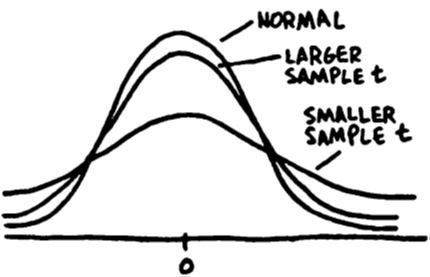
\includegraphics[width=.35\textwidth]{Images/TStudentNormal.png}
\end{center} 

\subsection{Intervalos de Confianza para la media}
Tenemos dos maneras de hacerlo:
\begin{enumerate}
    \item Si $n$ \emph{es grande} $\Rightarrows$ $(\mu - z_{\frac{1+\gamma}{2}}\frac{\sigma}{\sqrt{n}} ;\; \mu + z_{\frac{1+\gamma}{2}}\frac{\sigma}{\sqrt{n}} )$
    \item Si $n$ \emph{no es muy grande} $\Rightarrows$ $(\={X}_n - \frac{S}{\sqrt{n}}t_{n-1 \comma \frac{1+\gamma}{2}} ;\; \={X}_n + \frac{S}{\sqrt{n}}t_{n-1 \comma \frac{1+\gamma}{2}})$
\end{enumerate}
donde $t_{\nu \comma \alpha}$ se define como $P(T \leq t_{\nu \comma \alpha}) = \alpha$ si $T \sim t_{\nu \comma \alpha}$ (esta en tablas).
\\\underline{Observación}: $t_{\nu \comma \alpha} = -t_{\nu \comma 1 - \alpha}$
\\\\Tenemos dos tipos de intervalos: \emph{unilaterales} y \emph{bilaterales}
\subsubsection*{Unilaterales}
Puede ser el \emph{intervalo a derecha}:
\begin{equation*}
    \left(\={X}_n - \frac{S}{\sqrt{n}}t_{n-1 \comma \gamma} ;\; + \infty\right)
\end{equation*}
\begin{center}
        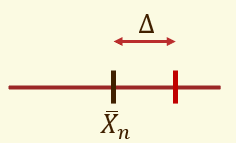
\includegraphics[width=.20\textwidth]{Images/IntSuperior.png}
\end{center} 
o el \emph{intervalo a izquierda}:
\begin{equation*}
    \left(-\infty ;\; \={X}_n + \frac{S}{\sqrt{n}}t_{n-1 \comma \gamma}\right)
\end{equation*}
\begin{center}
        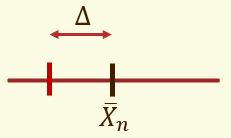
\includegraphics[width=.20\textwidth]{Images/IntInferior.png}
\end{center} 

\subsubsection*{Bilaterales}
\begin{equation*}
    \left(\={X}_n - \frac{S}{\sqrt{n}}t_{n-1 \comma \frac{1+\gamma}{2}} ;\; \={X}_n + \frac{S}{\sqrt{n}}t_{n-1 \comma \frac{1+\gamma}{2}}\right)
\end{equation*}
\begin{center}
        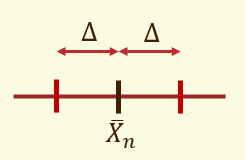
\includegraphics[width=.20\textwidth]{Images/IntBilateral.png}
\end{center} 

%-----------------------------
\newpage
\section{Prueba de Hipótesis}
Una \emph{prueba de hipótesis} es un procedimiento con el que se busca tomar una decisión sobre el \emph{valor de verdad de una hipótesis estadística}. 
Al hacerlo decidimos si rechazar o no esa hipótesis estadística.
\\Siempre tenemos dos hipótesis:
\begin{itemize}
    \item \underline{Hipótesis nula} ($H_0$): Es sostener lo que se dice o lo que se viene haciendo hasta ahora. Es decir, mantener el status quo. 
    \item \underline{Hipótesis alternativa} ($H_1$) : Es sostener lo opuesto a lo que se dice o cambiar lo que se viene haciendo hasta ahora.
\end{itemize}
\begin{tcolorbox}[title=Ejemplo]
Una agencia de protección al consumidor desea poner a prueba la afirmación de un fabricante de pinturas según la cual el tiempo medio de secado de su nueva pintura de secado rápido es de no más de 20 min. Entonces: 
\begin{itemize}
    \item $H_0$: El fabricante dice la verdad, por lo que el tiempo de secado es $\leq 20$.
    \item $H_1$: El fabricante miente, por lo que el tiempo de secado es $> 20$.
\end{itemize}
\end{tcolorbox}
Pero no podemos estar 100\% seguros de esto ya que el azar puede hacer que cometamos un error. Por lo que tenemos que tener en cuenta distintos casos:

\begin{table}[h]
\centering
\begin{tabular}{cc|cc|}
\cline{3-4}
\multicolumn{1}{l}{} & \multicolumn{1}{l|}{} & \multicolumn{2}{r|}{\cellcolor[HTML]{EFEFEF}Toma de decisión basada en $H_0$} \\ \cline{3-4} 
 &  & \multicolumn{1}{c|}{\cellcolor[HTML]{FFD43F}{\color[HTML]{000000} Aceptamos $H_0$}} & \cellcolor[HTML]{FFD43F}{\color[HTML]{000000} Rechazamos $H_0$} \\ \hline
\multicolumn{1}{|c|}{\cellcolor[HTML]{EFEFEF}{\color[HTML]{000000} }} & \cellcolor[HTML]{FFD43F}  $H_0$ verdadera & \multicolumn{1}{c|}{:D} & \cellcolor[HTML]{FD6864}{\color[HTML]{000000} \begin{tabular}[c]{@{}c@{}}ERROR\\ TIPO I \\ ($\alpha$)\end{tabular}} \\ \cline{2-4} 
\multicolumn{1}{|c|}{\multirow{-2}{*}{\cellcolor[HTML]{EFEFEF}{\color[HTML]{000000} \begin{tabular}[c]{@{}c@{}}Valor de verdad\\ de $H_0$\end{tabular}}}} & \cellcolor[HTML]{FFD43F} $H_0$ falsa & \multicolumn{1}{c|}{\cellcolor[HTML]{FD6864}{\color[HTML]{000000} \begin{tabular}[c]{@{}c@{}}ERROR\\ TIPO II \\ ($\beta$)\end{tabular}}} & :D ("potencia de la prueba") \\  \hline
\end{tabular}
\end{table}

\leavevmode\underline{Observación}: La \emph{potencia de la prueba} se puede calcular como: $1 - \beta$
\\Para esto, tenemos dos \textbf{estrategias}:
\begin{enumerate}
    \item Fijar, de antemano, un valor $\alpha_m$ como cota superior al ERROR TIPO I.
    \item Reportar qué tan probable es que una muestra haya sido tan contraria a $H_0$.
    Es decir, "asumiendo que $H_0$ es verdadera, ¿cuán probable es no observar lo observado?". Entonces, si es muy poco probable es "malo".
    A esto lo llamamos \emph{p-value} (es una medida de qué tan biased está nuestra $H_0$).
\end{enumerate}

\subsection{Definiciones}
\subsubsection*{Definición 1. Nivel de significación de la prueba}
Es la máxima probabilidad de cometer un error de tipo I que es posible admitir. Normalmente se fija en un valor $\alpha_m$.

\subsubsection*{Definición 2. Valor p/p-value}
El valor p se define como la probabilidad de que \emph{si la hipótesis nula es verdadera el estadístico de prueba dé tan mal o peor de lo que dio}.

\subsection{Pruebas de Hipótesis en $\=X_n$ con $\sigma$ conocido}
Dado $X \sim N(\mu \comma \sigma)$, con $\sigma$ conocido.
\\Además, como \emph{estadístico} se utilizará el valor medio: $\={X}_n \sim N(\mu \comma \frac{\sigma}{\sqrt{n}})$

\subsubsection{Prueba de cola derecha}
\begin{center}
        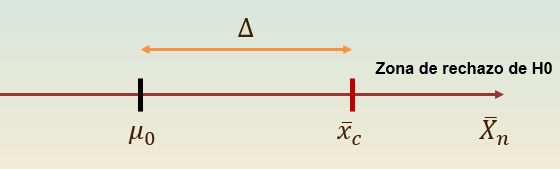
\includegraphics[width=.40\textwidth]{Images/ColaDerecha.png}
\end{center} 
Es cuando las hipótesis cumplen lo siguiente:
\begin{align*}
    H_0:& \mu \leq \mu_0 \\
    H_1:& \mu > \mu_0
\end{align*}
\subsubsection*{Estrategia 1}
Fijamos en $\alpha_m$ la \emph{máxima probabilidad de cometer un error de tipo I} que es posible admitir.
\\Entonces, rechazaremos $H_0$ si $\={X}_n$ es mas grande que $\={x}_c = \mu_0 + z_{1 - \alpha_m} \frac{\sigma}{\sqrt{n}}$. O lo que es lo mismo:
\begin{equation*}
    P_{\mu_0}(\={X}_n > \={x}_c) = 1 - \Phi\left(\frac{\={x}_c - \mu_0}{\sigma}\sqrt{n}\right) > \alpha_m
\end{equation*}
Si esto se cumple, entonces \emph{rechazaremos $H_0$}.
\\\\
Si $H_0$ fuera falsa, estaríamos cometiendo un error que depende de "qué tan falsa sea":
\begin{equation*}
    \beta(\mu) = P_\mu(\={X}_n \leq \={x}_c) = \Phi\left(\frac{\=x_c - \mu}{\sigma}\sqrt{n}\right)
\end{equation*}
Algunos \emph{valores conocidos} de $\beta$:
\begin{enumerate}
    \item $\beta(\mu_0) = 1 - \alpha_m$ 
    \item $1 - \beta(\mu_0)$ se llama potencia de la prueba
    \item $\beta(\={x}_c) = 0.5$
    \item $\lim_{\mu \rightarrow \infty} \beta(\mu) = 0$
\end{enumerate}

\subsubsection*{Estrategia 2}
Reportamos que tan probable es que una muestra haya sido tan contraria a $H_0$. O lo que es lo mismo:
\begin{equation*}
     \underbrace{P_{\mu_0}(\={X}_n > \={x}_{obs})}_{\text{p-value}} = 1 - \Phi\left(\frac{\={x}_{obs} - \mu_0 }{\sigma}\sqrt{n}\right) < \alpha_m
\end{equation*}
\leavevmode Si esto se cumple, entonces \emph{rechazaremos $H_0$}.


\subsubsection{Prueba de cola izquierda}
\begin{center}
        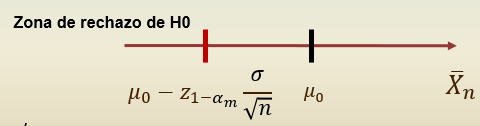
\includegraphics[width=.45\textwidth]{Images/ColaIzq.png}
\end{center} 
Es cuando las hipótesis cumplen lo siguiente:
\begin{align*}
    H_0:& \mu \geq \mu_0 \\
    H_1:& \mu < \mu_0
\end{align*}
\subsubsection*{Estrategia 1}
Fijamos en $\alpha_m$ la \emph{máxima probabilidad de cometer un error de tipo I} que es posible admitir.
\\Entonces, rechazaremos $H_0$ si $\={X}_n$ es mas chico que $\={x}_c = \mu_0 - z_{1 - \alpha_m} \frac{\sigma}{\sqrt{n}}$. O lo que es lo mismo:
\begin{equation*}
    P_{\mu_0}(\={X}_n \leq \={x}_c) = \Phi\left(\frac{\={x}_c - \mu_0 }{\sigma}\sqrt{n}\right) > \alpha_m
\end{equation*}
Si esto se cumple, entonces \emph{rechazaremos $H_0$}.
\\\\
Si $H_0$ fuera falsa, estaríamos cometiendo un error que depende de "qué tan falsa sea":
\begin{equation*}
    \beta(\mu) = P_\mu(\={X}_n > \={x}_c) = 1 - \Phi\left(\frac{\=x_c - \mu}{\sigma}\sqrt{n}\right)
\end{equation*}
Algunos \emph{valores conocidos} de $\beta$:
\begin{enumerate}
    \item $\beta(\mu_0) = 1 - \alpha_m$ 
    \item $1 - \beta(\mu_0)$ se llama potencia de la prueba
    \item $\beta(\={x}_c) = 0.5$
    \item $\lim_{\mu \rightarrow -\infty} \beta(\mu) = 0$
\end{enumerate}

\subsubsection*{Estrategia 2}
Reportamos que tan probable es que una muestra haya sido tan contraria a $H_0$. O lo que es lo mismo:
\begin{equation*}
     \underbrace{P_{\mu_0}(\={X}_n < \={x}_{obs})}_{\text{p-value}} = \Phi\left(\frac{\={x}_{obs} - \mu_0 }{\sigma}\sqrt{n}\right) < \alpha_m
\end{equation*}
\leavevmode Si esto se cumple, entonces \emph{rechazaremos $H_0$}.



\subsubsection{Prueba de dos colas}
\begin{center}
        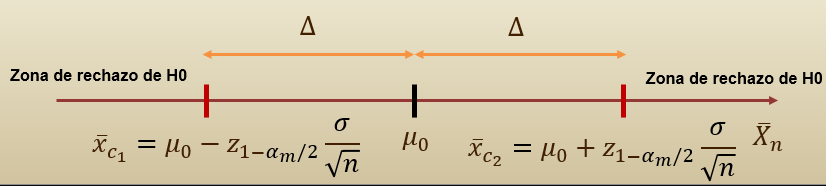
\includegraphics[width=.55\textwidth]{Images/DobleCola.png}
\end{center} 
Es cuando las hipótesis cumplen lo siguiente:
\begin{align*}
    H_0:& \mu = \mu_0 \\
    H_1:& \mu \neq \mu_0
\end{align*}
\subsubsection*{Estrategia 1}
Fijamos en $\alpha_m$ la \emph{máxima probabilidad de cometer un error de tipo I} que es posible admitir.
\\Entonces, rechazaremos $H_0$ si $\={X}_n$ es mas chica que $\={x}_{c_1} = \mu_0 - z_{1 - \alpha_m} \frac{\sigma}{\sqrt{n}}$ o mas grande $\={x}_{c_2} = \mu_0 + z_{1 - \alpha_m} \frac{\sigma}{\sqrt{n}}$. O lo que es lo mismo:
\begin{equation*}
    P_\mu(\={X}_n < \={x}_{c_1}  \cup \=X_n > \={x}_{c_2}) = 1 - \left[\Phi\left(\frac{\=x_{c_2} - \mu}{\sigma}\sqrt{n}\right) - \Phi\left(\frac{\=x_{c_1} - \mu}{\sigma}\sqrt{n}\right)\right] > \alpha_m
\end{equation*}
Si esto se cumple, entonces \emph{rechazaremos $H_0$}.
\\\\
Si $H_0$ fuera falsa, estaríamos cometiendo un error que depende de "qué tan falsa sea":
\begin{equation*}
    \beta(\mu) = P_\mu( \={x}_{c_1} \leq \={X}_n \leq \={x}_{c_2}) = \Phi\left(\frac{\=x_{c_2} - \mu}{\sigma}\sqrt{n}\right) - \Phi\left(\frac{\=x_{c_1} - \mu}{\sigma}\sqrt{n}\right)
\end{equation*}
Algunos \emph{valores conocidos} de $\beta$:
\begin{enumerate}
    \item $\beta(\mu_0) = 1 - \alpha_m$ (potencia de la prueba)
    \item $1 - \beta(\mu_0)$ se llama potencia de la prueba
    \item $\beta(\={x}_{c_1}) = \beta(\={x}_{c_1}) \approx 0.5$
    \item $\lim_{\mu \rightarrow \pm \infty} \beta(\mu) = 0$
\end{enumerate}

\subsubsection*{Estrategia 2}
Reportamos que tan probable es que una muestra haya sido tan contraria a $H_0$. O lo que es lo mismo:
\begin{equation*}
     \underbrace{P_{\mu_0}(|\={X}_n - \mu_0| > \Delta_{obs})}_{\text{p-value}} = 2\left[1 - \Phi\left(\frac{\Delta_{obs} \sqrt{n}}{\sigma}\right)\right] < \alpha_m
\end{equation*}
donde $\Delta_{obs} = |\=x_{obs} - \mu_0|$.
\\Si esto se cumple, entonces \emph{rechazaremos $H_0$}.

\subsection{Pruebas de Hipótesis en $Z$ con $\sigma$ conocido}
Usando $Z = \frac{(\=X_n - \mu_0)\sqrt{n}}{\sigma}$ obtenemos un \emph{estadístico de muestra adimensional}. 
\\Además sabemos que para $n$ grande se cumple:
\begin{equation*}
    \hat{p} \sim N \left(p \comma \sqrt{\frac{p(1-p)}{n}} \right)
\end{equation*}
Luego, podemos hacer lo mismo que hicimos para $\=X_n$ en la proporción.
\subsubsection{Prueba de cola derecha}
\begin{center}
        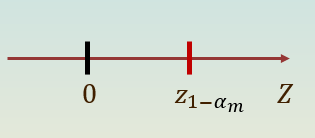
\includegraphics[width=.30\textwidth]{Images/colaDerAdimensional.png}
\end{center} 
Es cuando las hipótesis cumplen lo siguiente:
\begin{align*}
    H_0:& p \leq p_0 \\
    H_1:& p > p_0
\end{align*}
Además, \textbf{p-value} $= 1 - \Phi(|z_{obs}|)$

\subsubsection{Prueba de cola izquierda}
\begin{center}
        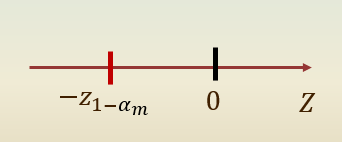
\includegraphics[width=.33\textwidth]{Images/ColaIzqAdimensional.png}
\end{center} 
Es cuando las hipótesis cumplen lo siguiente:
\begin{align*}
    H_0: p \geq p_0 \\
    H_1: p < p_0
\end{align*}
Además, \textbf{p-value} $= \Phi(|z_{obs}|)$

\subsubsection{Prueba de dos colas}
\begin{center}
        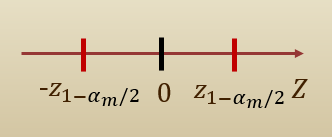
\includegraphics[width=.30\textwidth]{Images/DobleColaAdimensional.png}
\end{center} 
Es cuando las hipótesis cumplen lo siguiente:
\begin{align*}
    H_0:& p = p_0 \\
    H_1:& p \neq p_0
\end{align*}
Además, \textbf{p-value} $= 2[1 - \Phi(|z_{obs}|)]$

\newpage
\subsection{Pruebas de Hipótesis en $\=X_n$ con $\sigma$ desconocido}
Dada $X \sim N(\mu \comma \sigma)$. Se considera una muestra aleatoria $\{X_1 \comma ... \comma X_n\}$ de tamaño $n$ de $X$.
\\Tomamos $T = \frac{\=X - \mu}{S} \sqrt{n} \sim t_{n-1}$
\begin{center}
        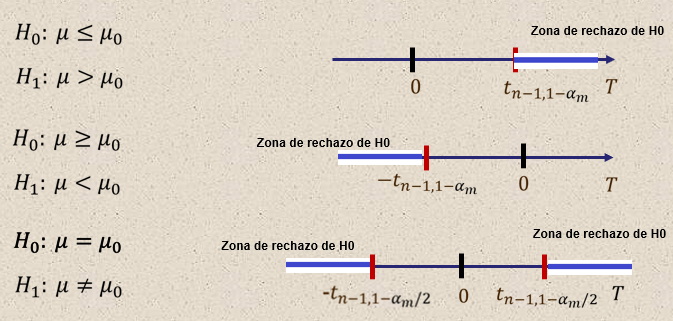
\includegraphics[width=.50\textwidth]{Images/PrubasHipStudent.png}
\end{center} 
\underline{Observación}: Si comparamos los fractiles de $t$ y la \emph{normal estándar}, entonces se puede ver que: 
\begin{equation*}
    t_{n-1 \comma w} > z_w \; \forall w \in (0 \comma 1)
\end{equation*}

%----------------------------------------------
\newpage
\section{Procesos Estocásticos}
Un proceso estocástico es un proceso/sistema que se desarrolla/evoluciona en el tiempo (y/o espacio) mientras que pasa por fluctuaciones al azar.
\\En cada instante/posición se tiene una \textbf{va} cuyo valor es \textbf{estado del proceso} y cuya distribución de probabilidades \textbf{puede cambiar con el tiempo/posición}.

\subsection{Definiciones}
\subsubsection*{Definición 1. Proceso Estocástico}
Conjunto de variables aleatorias $X = \{ X(t) : t \in T\}$

\subsubsection*{Definición 2. Espacio del Parámetro}
Es la $T$ que aparece en $X = \{ X(t) : t \in T\}$

\subsubsection*{Definición 3. Espacio de Estados}
Es la unión de los recorridos de las variables $X(t)$. 
\\\underline{Notación}: $E$

\begin{tcolorbox}[title=Ejemplos]
\begin{itemize}
    \item  $X(t)$: La temperatura corporal tomada en la axila izquierda en el instante $t$.
    \\$\Rightarrows T = \reales_{\geq 0} \comma E \subset \reales$
    \item $N(t)$: Número de personas que han arribado a la fila de un banco hasta el instante $t$.
    \\$\Rightarrows T = \reales_{\geq 0} \comma E \subset \naturales_0$
\end{itemize}
\underline{Observación}: Notemos que en el primer caso $T$ y $E$ son \emph{continuos}, mientras que en el segundo $T$ es continuo pero $E$ es \emph{discreto}.
\end{tcolorbox}

\subsubsection*{Definición 4. Incremento Estacionario}
Se dice que un proceso estocástico tiene \emph{incrementos estacionarios} sii:
\begin{equation*}
    P(X(t_2 + \tau) - X(t_1 + \tau) \leq x) = P(X(t_2) - X(t_1  )) \;\; \forall t_1 < t_2 \comma \forall \tau \comma \forall x
\end{equation*}
Es decir, \emph{la distribución de incrementos "no depende" del tiempo}.
\\Por ejemplo, la caminata aleatoria es de incrementos estacionarios.

\subsubsection*{Definición 5. Incremento Independientes}
Se dice que un proceso estocástico tiene \emph{incrementos independientes} sii:
\begin{equation*}
    \forall n \comma \forall (l_1 \comma u_1) \comma ... \comma (l_n \comma u_n) \text{ con } l_i < u_i \text{ y } (l_k \comma u_m) \cap (l_k \comma u_k) = \varnothing \text{ si } m \neq k
\end{equation*}
se cumple que las variables aleatorias: 
\begin{equation*}
    \Delta_i = X(u_i) - X(l_i) \text{ son independientes entre sí}
\end{equation*}
\\Luego, podemos describir al proceso como \emph{una suma de incrementos independientes} de la siguiente manera:
\begin{equation*}
    l_i = u_{i-1} \text{ y } X(u_n) - X(l_1) = \sumatoria{i = 2}{n} \Delta_i
\end{equation*}
Por ejemplo, la caminata aleatoria es de incrementos independientes.

\subsubsection*{Definición 5. Proceso de Conteo}
Se dice que un proceso estocástico $N(t)$ \emph{es de conteo} sii: 
\begin{enumerate}
    \item $N(0) = 0$
    \item $N(t) \geq 0 \;\; \forall t \geq 0$
    \item $s < t \Rightarrows N(s) \leq N(t)$
    \item $E = \naturales_0$
\end{enumerate}
\underline{Observación}: $N(t) - N(s)$ son los eventos que ocurrieron \emph{después de s pero antes de t}.

\subsubsection*{Definición 6. Cadenas homogénes}
Es cuando en una \emph{cadena de Markov}, las probabilidades de transición \underline{no} dependen del tiempo:
\begin{equation*}
    p_{ij}(n) = p_{ij}
\end{equation*}

\subsection{Procesos de Poisson}
Se dice que un \textbf{proceso estocástico de conteo} $N(t)$ es un \emph{proceso de Poisson de parámetro $\lambda$} sii:
\begin{enumerate}
    \item Tiene \textbf{incrementos independientes}.
    \item Los \textbf{incrementos son estacionarios}.
    \item La probabilidad de que exactamente \textbf{un evento} ocurra en un intervalo de tiempo de longitud $h$ es $\lambda h + o(h)$
    \item La probabilidad de que \textbf{más de un evento} ocurra en un intervalo de tiempo de longitud $h$ es $o(h)$
\end{enumerate}

\subsubsection*{Características de los Procesos de Poisson}
\begin{enumerate}
    \item La probabilidad de que en un intervalo de tiempo $(0 \comma t)$ hayan ocurrido $n$ eventos del proceso de Poisson es:
    \begin{equation*}
        p_n(t + h) = P(N(t + h) = n) = \frac{(\lambda t)^n}{n!} e^{-\lambda t}
    \end{equation*}
    entonces $N(t) \sim Poisson(\lambda t)$
    \item Los tiempos entre eventos ($\tau$) tienen distribución exponencial.
    \\Los tiempos entre eventos ($\tau$) son independientes entre sí.
    \begin{equation*}
        \Rightarrows \text{Los tiempos entre eventos ($\tau$) son variables iid con distribución exponencial de parámetro $\lambda$}
    \end{equation*}
    \item El tiempo $S_k$ hasta la ocurrencia del evento $k$ es una vac con distribución $Gamma$ de parámetros $k$ y $\lambda$. Luego, se verifica que:
    \begin{equation*}
        P(S_k < t) = P(N_t \geq k) = 1 - P(N_t < k)
    \end{equation*}
\end{enumerate}

\subsection{Cadenas de Markov}
Se dice que un proceso estocástico es un proceso de Markov sii $\forall n \comma \forall t_1 < t_2 < ... < t_n \comma \forall x$, se cumple que:
\begin{equation*}
    P(X(t_n) \leq x | X(t_{n-1}) \comma ... \comma X(t_1)) = P(X(t_n) \leq x | X(t_{n-1}))
\end{equation*}
es decir, \emph{sólo importa el valor más reciente}.
\\De esta manera, se llama \textbf{cadena de Markov} a un proceso de Markov que tiene un \emph{spacio de parámetro discreto}: $T = \naturales^0$, 
y (en nuestro caso) \emph{un espacio de estados discreto} $E = \{e_1 \comma e_2 \comma ... \}$.
\subsubsection*{Observaciones}
Una cadena de Markov $\{X(n)\}_{n \in \naturales^0}$ queda completamente descripta por:
\begin{enumerate}
    \item La distribución de probabilidades del estado inicial.
    \begin{align*}
        p_j(0) &= P(X(0) = e_j) \\
        \sumatoria{j}{} p_j(0) &= 1
    \end{align*}
    que tambien se puede representar como \emph{vector de probabilidades}:
    \begin{equation*}
        \Vec{p}(n) = (p_1(n) \;\; p_2(n) \;\; ... )
    \end{equation*}
    \item Las probabilidades de transición entre cada par de estados.
    \begin{equation*}
    p_{ij}(n) = P(X(n+1) = e_j | X(n) = e_j)
    \end{equation*}
    que también se pueden representar como \emph{matriz de probabilidades de transición de un sólo paso}:
        \[
          \mathbb{P}(n) =
          \left[ {\begin{array}{cccc}
            p_{11} & p_{12} & \cdots \\
            p_{21} & p_{22} & \cdots \\
            \vdots & \vdots & \ddots \\
          \end{array} } \right]
        \]
    Esto último se puede ver gráficamente como un grafo dirigido de la siguiente manera:
    \begin{center}
            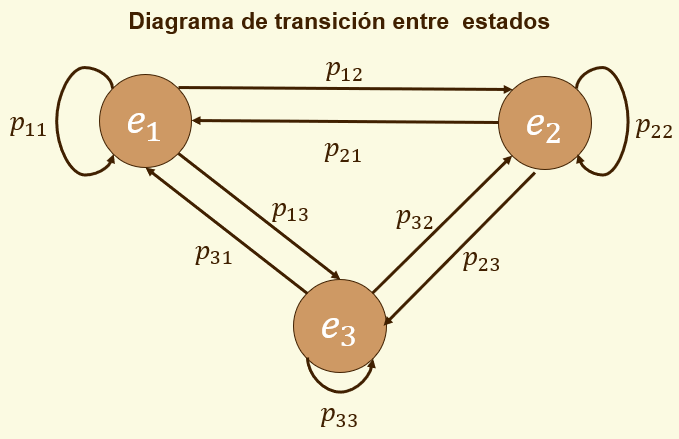
\includegraphics[width=.40\textwidth]{Images/DiagramaTransEstados.png}
    \end{center} 
\end{enumerate}

\subsubsection{Ecuación de Chapman-Kolmogorov}
\underline{\emph{Forma vectorial}}: $p_j(n+1) = \sumatoria{i}{} p_i(n) p_{ij}(n)$
\\\\\underline{\emph{Forma matricial}}: $\Vec{p}_j(n+1) = \Vec{p}(n) \mathbb{P}(n)$
\\\\ Si la \emph{cadena fuese homogénea}, entonces:  $\Vec{p}(n+1) = \Vec{p}(0) \mathbb{P}^n$ 
por lo que la \textbf{matriz de probabilidades en $k$ pasos} se obtendría como: $\mathbb{P}^{(k)} = \mathbb{P}^k$

\subsubsection{Probabilidad a largo plazo/Distribución estacionaria}
\begin{equation*}
    \Vec{\pi} = \lim_{n \rightarrow \infty} \Vec{p}(n) = \left[\lim_{n \rightarrow \infty}\Vec{p}(n)\right] \mathbb{P} = \Vec{\pi} \mathbb{P}
\end{equation*}
\underline{Observaciones}
\begin{enumerate}
    \item Si existe $\Rightarrows$ se corresponde con un autovector a izquierda correspondiente al autovalor 1 de $\mathbb{P}$.
    \item No toda distribución que satisface la ecuación es una distribución estacionaria.
\end{enumerate}
La \textbf{condición suficiente para la existencia de una distribución estacionaria} es:
\\\emph{"Dada una cadena de Markov, si $\exists k \tq \mathbb{P}^k$ tiene todos sus elementos positivos $\Rightarrows$ existe una distribución de probabilidad estacionaria"}.


\end{document}